\documentclass[11pt]{article}
\usepackage[a4paper,margin=2.2cm]{geometry}
\usepackage{lmodern}
\usepackage[T1]{fontenc}
\usepackage{microtype}
\usepackage{amsmath}
\usepackage{amssymb}
\usepackage{booktabs}
\usepackage{tabularx}
\usepackage{multirow}
\usepackage{makecell}
\usepackage{placeins}
\usepackage{float}
\usepackage{xltabular}
\usepackage{colortbl}
\usepackage{enumitem}
\usepackage{caption}
\usepackage[dvipsnames]{xcolor}
\usepackage{tikz}
\usetikzlibrary{positioning,arrows.meta,fit,backgrounds,calc,shapes.geometric}
\usepackage[colorlinks=true,linkcolor=MidnightBlue,urlcolor=MidnightBlue,citecolor=MidnightBlue]{hyperref}

\setlist{itemsep=2pt,topsep=4pt}
\newcommand{\dq}{\textsc{DocQuorum}}
\newcommand{\nohyph}{\hyphenpenalty=10000 \exhyphenpenalty=10000 \raggedright}
\newcolumntype{Y}{>{\raggedright\arraybackslash}X}
\newcolumntype{L}[1]{>{\raggedright\arraybackslash}p{#1}}
\definecolor{fe}{HTML}{DCEBFA}
\definecolor{rd}{HTML}{E3F4E1}
\definecolor{ck}{HTML}{FFF1D6}
\definecolor{cs}{HTML}{F6E0F0}
\definecolor{ln}{HTML}{4A4A4A}

\title{\dq: Agentic Document Extraction\\by a Quorum of Grounded Readings}
\author{Ashutosh Dayal}
\date{28 September 2026}

\begin{document}
\maketitle

\begin{abstract}
\noindent
\dq{} turns a document --- a PDF of one to a few hundred pages, a scan, or a photo --- into JSON
that follows a user-given schema. It combines three ideas. \emph{A reader agent that plans by
budget}: it reads the whole document in one model call when it fits, splits the
\emph{schema} when the schema is what does not fit, and reads windows or page chunks
otherwise, checking every reply for truncation, empty answers and skipped fields and acting
again when it finds one. \emph{Ground, don't ask}: repair and check the output against the
document's own text --- record counts, printed page numbers, quotation marks, rows copied
between tables --- instead of asking the model to check itself. \emph{Quorum}: when several
independent readings of a document are available, keep the one the others agree with most.
With open-weight models on a single GPU, \dq{} scores 95.25 on ExtractBench (3rd of 45
leaderboard entries, behind two commercial systems) and 82.37 on UNIKIE-BENCH with six readings
from three open models, tying the best published system.
\end{abstract}

% ---------------------------------------------------------------------------
\section{The task}
The input is a document and a \emph{schema}: a JSON Schema (or a JSON template with empty
values) naming the fields to extract, usually with instructions in the field descriptions ---
label aliases, where on the page to look, what not to confuse the field with, and the format of
the answer. The output is one JSON object. Scoring is strict: each extracted value must match
the annotated value exactly (after light normalisation), rows of repeated tables are paired one
to one, and a missing field counts as an error.

Figure~\ref{fig:task} shows one ExtractBench task in full: a one-page purchase order, the schema
it comes with, and the answer. Even this page is not a lookup. The purchase-order number is
printed three times (a barcode, the header, the footer note) and the page's own title,
``Requisition Purchase Order'', is not the requisition number: that sits in a row of column
headings (vendor phone number, vendor email, vendor number, requisition number, \ldots) with its
value, 12602080, one line below. The only other amount on the page, ``a maximum of: \$0.00'' in the
approval text, is not the total. And the schema asks for normalised values: the printed
``08/28/2025'' becomes \texttt{"2025-08-28"} and ``\$6,721.8000'' becomes \texttt{6721.8}.

\begin{figure}[t]
\centering
\begin{minipage}[t]{0.405\textwidth}\vspace{0pt}
\fbox{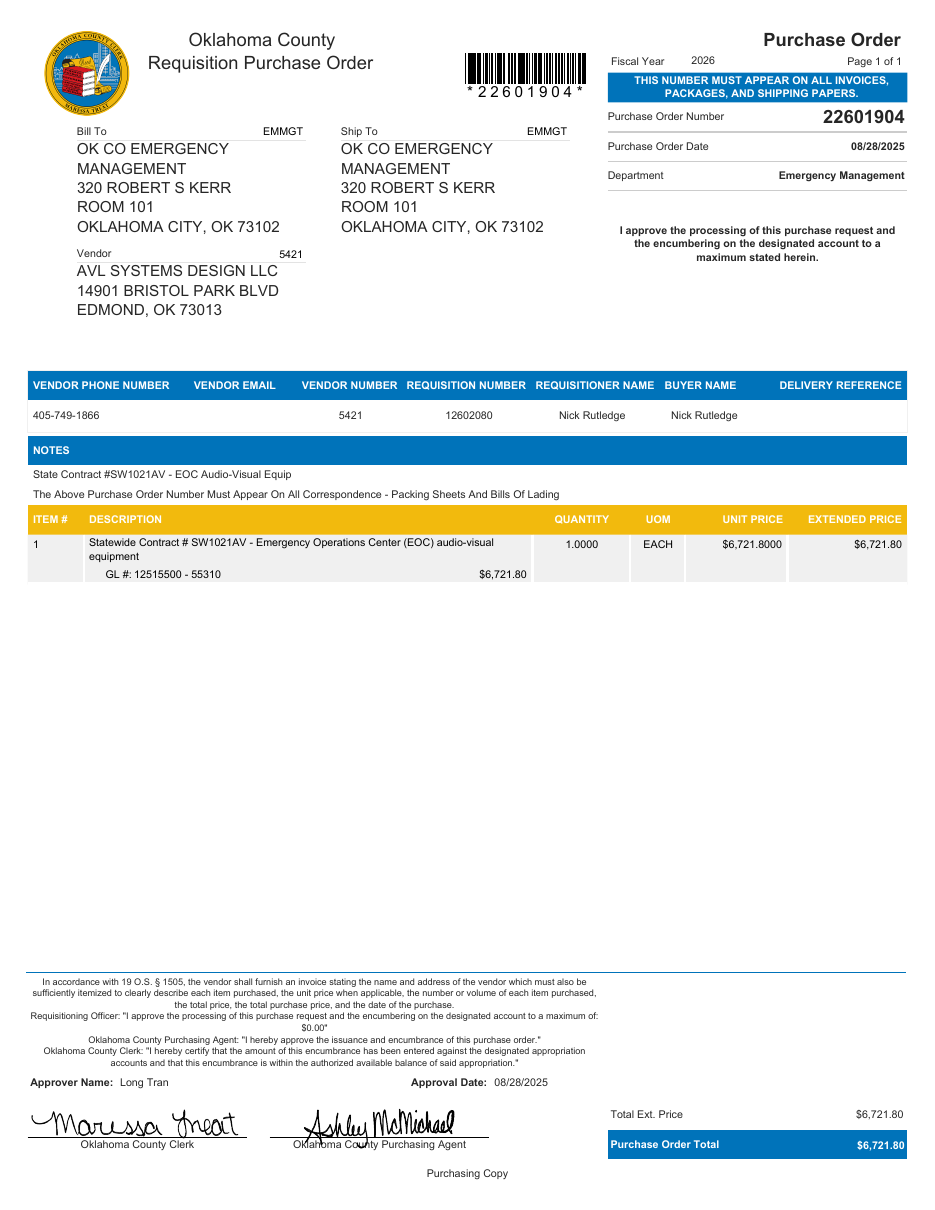
\includegraphics[width=0.97\linewidth]{fig/okpo-1.png}}\\[3pt]
{\footnotesize\raggedright\textbf{(a) Document}: a one-page digital PDF (made by software, so its text is exact), \texttt{oklahoma\_county\_\allowbreak
purchase\_order\_\allowbreak avl\_systems} (ExtractBench, short split).\par}
\end{minipage}\hfill
\begin{minipage}[t]{0.575\textwidth}\vspace{0pt}
{\footnotesize\textbf{(b) Schema} (4 of 12 fields, descriptions abridged; 14,292 characters in all)}
\scriptsize
\begin{verbatim}
"po_number": {"anyOf": [{"type":"string"},{"type":"null"}],
  "description": "The purchase order's own unique identifier,
   taken ONLY from a field explicitly labeled with a PO-number
   alias ... Do NOT confuse with: the requisition_number, the
   contract/bid number, ... the vendor number ..."},
"requisition_number": { ... "Label aliases: 'Requisition
   Number', 'Requisition Purchase Order', 'Req #'. ... Location:
   header, often directly under the PO number. Return null if
   no field is explicitly labeled as a requisition number"},
"line_items": {"type": "array", "description": "Every ordered
   line item from THIS purchase order's OWN line-item table ...
   EXCLUDE: empty filler rows that show '$0.00' ...; subtotal/
   Total/Grand Total rows ...", "items": {"properties": {
   "line_no", "description", "quantity", "unit_of_measure",
   "unit_price", "start_date", "end_date", "extended_price"}}},
"total_amount": { ... "as a number (strip currency symbol and
   thousands separators; '$39,360.00' -> 39360.0) ..."}
\end{verbatim}
\vspace{-2pt}
{\footnotesize\textbf{(c) Output} (the annotated answer; four fields shown abridged as \ldots)}
\scriptsize
\begin{verbatim}
{"po_number": "22601904", "requisition_number": "12602080",
 "po_date": "2025-08-28",
 "buyer": {"name": "Oklahoma County",
           "department": "Emergency Management"},
 "requisitioner": "Nick Rutledge",
 "buyer_contact": "Nick Rutledge",
 "vendor": {"name": "AVL SYSTEMS DESIGN LLC",
   "address": "14901 BRISTOL PARK BLVD EDMOND, OK 73013",
   "vendor_number": "5421", "contact": "405-749-1866"},
 "ship_to": "...", "bill_to": "...",
 "line_items": [{"line_no": 1, "description": "Statewide
   Contract # SW1021AV - Emergency Operations Center (EOC)
   audio-visual equipment", "quantity": 1.0,
   "unit_of_measure": "EACH", "unit_price": 6721.8,
   "start_date": null, "end_date": null,
   "extended_price": 6721.8}],
 "total_amount": 6721.8, "currency": "USD"}
\end{verbatim}
\end{minipage}
\caption{One ExtractBench task. \dq{}'s answer matches (c) except \texttt{buyer\_contact} and
\texttt{vendor.contact}, which it returns as null: score 91.3. Before the reader agent learned to
re-read a reply that leaves schema keys out (\S\ref{sec:agent}), every reading returned
\texttt{requisition\_number} as a missing key.}
\label{fig:task}
\end{figure}

\noindent Across the benchmark the difficulty grows along four axes:
\begin{itemize}
  \item \textbf{Length.} A 59-page unclaimed-property register holds 26,725 records and a
        114-page creditor list 7,554; no single model reply can hold them.
  \item \textbf{Huge schemas.} A tax-return schema is 550,000 characters even written
        compactly --- larger than the model's 131k-token context.
  \item \textbf{Scans and layouts.} Image-only pages, a register printed in seven columns,
        ruled tables of identical rows.
  \item \textbf{Exactness.} ``Bachelor\textquotesingle s'' (straight apostrophe) is wrong when
        the page prints ``Bachelor\textquoteright s'' (curly).
\end{itemize}

% ---------------------------------------------------------------------------
\section{The pipeline at a glance}

\begin{figure}[t]
\centering
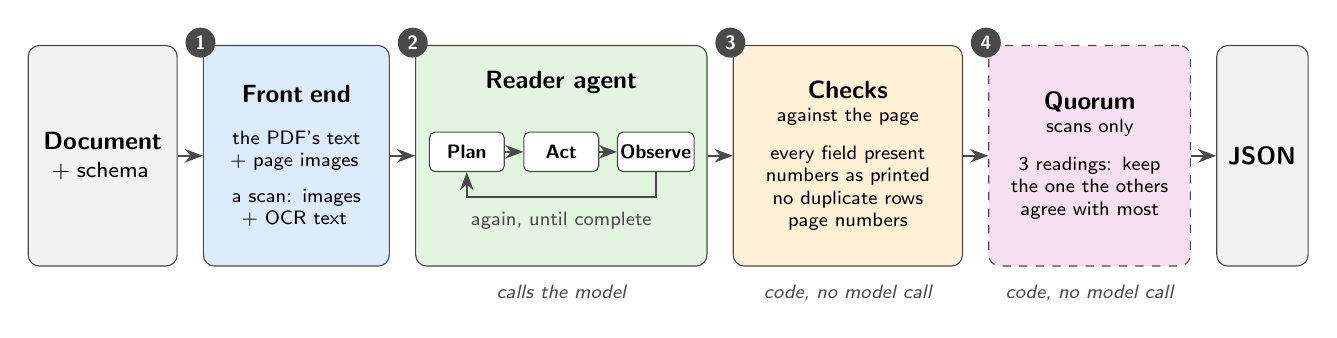
\begin{tikzpicture}[
  font=\sffamily,
  arr/.style={-{Stealth[length=2.3mm]}, line width=0.8pt, draw=ln},
  st/.style={draw=ln, rounded corners=4pt, align=center, minimum height=2.8cm, inner sep=3pt,
             font=\sffamily\scriptsize, execute at begin node=\nohyph\centering,
             anchor=west},
  io/.style={st, fill=gray!10, text width=1.25cm},
  ttl/.style={font=\sffamily\small\bfseries},
  ln1/.style={font=\sffamily\footnotesize, text=ln},
  num/.style={circle, fill=ln, text=white, font=\sffamily\bfseries\scriptsize, inner sep=0pt,
              minimum size=0.38cm},
  lp/.style={draw=ln, rounded corners=2pt, fill=white, font=\sffamily\scriptsize\bfseries,
             minimum width=0.95cm, minimum height=0.5cm, inner sep=1pt},
]
\node[io, text width=1.68cm] (in) at (0,0) {{\small\bfseries Document}\\[2pt]{\footnotesize + schema}};
\node[st, fill=fe, text width=2.15cm] (fe) at ([xshift=0.32cm]in.east)
  {{\small\bfseries Front end}\\[7pt] the PDF's text\\ + page images\\[5pt] a scan: images\\ + OCR text};
\node[st, fill=rd, minimum width=3.7cm] (ag) at ([xshift=0.32cm]fe.east) {};
\node[ttl, anchor=north] at ([yshift=-6pt]ag.north) {Reader agent};
\node[lp] (ac) at ([yshift=0.05cm]ag.center) {Act};
\node[lp] (pl) at ([xshift=-1.2cm]ac) {Plan};
\node[lp] (ob) at ([xshift=1.2cm]ac) {Observe};
\draw[arr] (pl) -- (ac);
\draw[arr] (ac) -- (ob);
\draw[arr] (ob.south) -- ++(0,-0.32) -| (pl.south);
\node[font=\sffamily\scriptsize, text=ln, anchor=north] at ([yshift=-0.38cm]ac.south) {again, until complete};
\node[st, fill=ck, text width=2.7cm] (ck) at ([xshift=0.32cm]ag.east)
  {{\small\bfseries Checks}\\ against the page\\[6pt] every field present\\ numbers as printed\\ no duplicate rows\\ page numbers};
\node[st, fill=cs, text width=2.35cm, dashed] (qu) at ([xshift=0.32cm]ck.east)
  {{\small\bfseries Quorum}\\ scans only\\[6pt] 3 readings: keep\\ the one the others\\ agree with most};
\node[io, text width=0.95cm] (out) at ([xshift=0.32cm]qu.east) {{\small\bfseries JSON}};
\foreach \a/\b in {in/fe, fe/ag, ag/ck, ck/qu, qu/out} {\draw[arr] (\a.east) -- (\b.west);}
\foreach \n/\k in {fe/1, ag/2, ck/3, qu/4} {\node[num] at ([xshift=-0.03cm, yshift=0.03cm]\n.north west) {\k};}
\node[font=\sffamily\scriptsize\itshape, text=ln, anchor=north] at ([yshift=-3pt]ag.south) {calls the model};
\node[font=\sffamily\scriptsize\itshape, text=ln, anchor=north] at ([yshift=-3pt]ck.south) {code, no model call};
\node[font=\sffamily\scriptsize\itshape, text=ln, anchor=north] at ([yshift=-3pt]qu.south) {code, no model call};
\end{tikzpicture}
\caption{\dq{} end to end. (1) The front end prepares what the model sees: a PDF's own text and
its page images, or for a scan the images and their OCR text. (2) The reader agent plans the
largest piece that fits one model call, acts, observes the reply, and acts again until it is
complete. (3) Code checks the answer against the page. (4) A scan is read three ways, and the
quorum keeps the reading the other two agree with most. Section~\ref{sec:stages} explains each step
with ExtractBench examples.}
\label{fig:pipeline}
\end{figure}

\noindent Figure~\ref{fig:pipeline} is the whole system. One module is an agent in the full
sense: the \emph{reader agent} (2) chooses its next action --- one call, a part of the schema, a
window of pages, a page chunk --- from a budget, calls the model, observes the reply
(\texttt{finish\_reason}, an empty list, keys the reply left out) and acts again. Its
\emph{tools} are the front end (1): the text layer, page images, the parser and two layout
readers. What the agent returns passes through deterministic code: repairs and checks (3), and,
for scans and photos, the quorum (4).

Table~\ref{tab:walk} follows six ExtractBench documents through Figure~\ref{fig:pipeline}. The
purchase order of Figure~\ref{fig:task} appears twice: the benchmark also contains it as a
degraded scan with no text layer, which sends it down the other branch.

\begin{table}[H]
\centering\small
\begin{tabularx}{\textwidth}{@{}L{3.55cm}Yr@{}}
\toprule
\textbf{Document} (ExtractBench) & \textbf{Route through Figure~\ref{fig:pipeline}} & \textbf{Score} \\
\midrule
Oklahoma purchase order, 1 page, digital PDF (Figure~\ref{fig:task}) &
text layer $\rightarrow$ reader agent: one whole-document call with the text layer and the page at
220\,dpi; the reply left schema keys out (among them the requisition number), so the agent read it
again with every key required $\rightarrow$ checks $\rightarrow$ JSON & 91.3 \\\addlinespace[4pt]
the same purchase order as a degraded scan (\texttt{\_corrupted}) &
no text layer $\rightarrow$ three readings: the agent on the page image, the agent on the MinerU
parse, the one-shot reader $\rightarrow$ checks on each $\rightarrow$ quorum: agreement 0.935,
0.935 and 0.957, so it keeps the one-shot reading & 78.3 \\\addlinespace[4pt]
W-14 well form 58025, 1 page, scan with OCR text &
text layer found, but it is OCR text over a scan $\rightarrow$ reader agent: the text is labelled
machine-read and the page image at 220\,dpi decides where they disagree; the 180,285-character
schema still fits one call (above 60,000 characters it is sent compact and decoded as plain
JSON rather than under a grammar) & 98.4 \\\addlinespace[4pt]
bar-lev-2022 tax return, 25 scanned pages &
no text layer, too long for one call's images; the schema (537,786 characters) does not fit
either $\rightarrow$ reader agent on the parse: the schema split into groups, each read in windows
of $\le$\,8 pages with their page images and OCR text; windows merged $\rightarrow$ checks & 98.2 \\\addlinespace[4pt]
unclaimed-property register, 59 pages, 26,725 records &
page geometry: at least three text columns of near-equal width (seven here) $\rightarrow$ column-flow
reader: each column cut out and read top to bottom, one call per column $\rightarrow$ checks & 98.2 \\\addlinespace[4pt]
ftx creditor list, 114 scanned pages, 7,554 rows (\texttt{\_corrupted}) &
no text layer, and its parsed tables map onto the schema's fields ($\ge$\,90\% of their rows
convert) $\rightarrow$ ruled-table reader: rows counted from the rules, each band of $\le$\,12 rows
read with its exact count $\rightarrow$ checks, e.g.\ identical ``NAME ON FILE'' records capped at
the count each page prints & 95.4 \\\addlinespace[4pt]
\bottomrule
\end{tabularx}
\caption{Six documents through the pipeline (score: the benchmark's value F1, $\times$100).}
\label{tab:walk}
\end{table}

% ---------------------------------------------------------------------------
\section{The stages}
\label{sec:stages}
Every step below was added because a document in ExtractBench came out wrong without it. Each
table row names that document, says what its page shows and what came out, and gives the effect
measured when the step was added. Scores are the benchmark's value F1 ($\times$100); ``short'',
``medium'' and ``long'' are its three groups of 252, 98 and 20 documents. The prompts are in
Appendix~\ref{app:prompts}.

\subsection{Front end: what the agent is shown}
A PDF is one of three kinds, and the front end first tells them apart from the file itself:
\begin{itemize}
  \item a \textbf{digital PDF}, made by software (exported from a word processor, printed from a
        web page): the text embedded in it --- its \emph{text layer} --- holds the exact
        characters;
  \item a \textbf{scanned PDF with OCR text}: page images, plus a text layer that a recognition
        program read from them, which can contain misreads;
  \item a \textbf{scan or photo without text}: page images only.
\end{itemize}
A text layer is read with \texttt{pdftotext -layout}, which keeps the page's columns aligned.
Scans without text are read by MinerU2.5, a 1.2B-parameter document parser that returns tables
as cells, so an empty column cannot shift every later value into the wrong column. Page images
go with the text whenever the document is short enough: up to 12 pages, each at 220~dpi, and
scans of 13--24 pages as pairs of pages side by side.

A digital PDF is not sent through the parser, even when it holds tables: its text layer
already has the exact characters with the table's columns kept aligned, and for documents of up
to 12 pages the page images show the table's lines. Reading digital PDFs through the parser was
measured and lost: on the 252 short documents the parser reading scored 94.50 against 94.87 for
the text-layer reading, and letting the quorum choose between the two lowered digital PDFs (a
census table 98.5 $\rightarrow$ 68.0; keeping the text reading: short 95.06 $\rightarrow$
95.14). Two table layouts that defeat the text layer get their own treatment below:
side-by-side tables, and registers printed in several columns.

\begingroup\small
\begin{xltabular}{\textwidth}{@{}L{2.9cm}YY@{}}
\caption{Front-end steps and the ExtractBench documents that called for them.}\label{tab:fe}\\
\toprule
\textbf{Step} & \textbf{Where it went wrong without it} & \textbf{Effect} \\
\midrule
\endfirsthead
\toprule
\textbf{Step} & \textbf{Where it went wrong without it} & \textbf{Effect} \\
\midrule
\endhead
\bottomrule
\endlastfoot
tell the kinds of PDF apart; label OCR text as machine-read &
a scanned statement of share holdings with OCR text: the text says ``550000'' where the page
shows 55.0000 shares (OCR dropped the decimal point). The text was presented as exact, so the
model copied 550000 &
the text of a scan is now labelled machine-read and the model told to trust the page image
where they differ: +0.25 on the 84 scanned PDFs with OCR text (two holdings statements +10
each; four documents $-$2 to $-$4) \\
page images at 220\,dpi (was 150\,dpi) &
scanned forms with handwritten entries and tick boxes (insurance claims remittances, oil-well
H-forms): at 150\,dpi small handwriting was misread and ticks were missed &
+0.62 on 225 documents read both ways (80 better, 38 worse); scans without any text +2.3;
claims remittances +12 each \\
page images for the parser at full resolution &
the Oklahoma unclaimed-property register prints about 460 names and addresses per page in
small type. Rendered at 144\,dpi and shrunk to 2.2 megapixels, the parser read ``PO BOX 757''
as ``POBOX757'' and ``WALKER DEBBIE'' as ``WAI KER DEBBIE''. Worse, extra resolution went only
to pages whose PDF holds much text --- and a scan holds none, so the documents that depend
most on the parser got the coarsest images &
small print and every scan are now rendered at 300\,dpi (up to 16 megapixels) \\
count pages from the PDF itself &
pages were counted by splitting the extracted text at its page-break characters, and the
extraction tool puts one after the last page too, so every PDF looked one page longer than it
is. A later rule --- use the parser's text only if at least 90\% of the pages were parsed ---
then failed for every document of 8 pages or fewer: the parser's text was silently ignored for
243 of the 252 short documents, all 94 scans among them &
with the parser's text really used as the second reading of scans: short 95.34 $\rightarrow$
95.99 \\
split side-by-side tables &
the iShares bond-fund report prints its holdings as two tables side by side (Security, Par,
Value --- twice). The parser glued them into one six-column table, and Qwen3-VL-8B and -32B both
returned no holdings for those pages; the PDF's own text interleaves the two tables on every
line &
cut where the column header repeats (three or more column names, repeated); applies to two
documents only \\
column-flow reader &
the same Oklahoma register prints seven alphabetical columns per page, like a newspaper. Read
across the page, every line mixes seven different people; read as one page image, the small
print is misread (``RT 1 BOX 220'' as ``BT 1 ROY 320'') &
each column cut out and read on its own: 20.92 $\rightarrow$ 91.64 (98.2 with the current
model); the OFAC sanctions list 87.0 $\rightarrow$ 89.0. Chosen from the page geometry alone (at
least three columns of near-equal width), which picks these two of the 20 long documents and
none of 45 others checked \\
ruled-table reader &
the FTX creditor list (114 scanned pages; redacted creditors all printed as ``NAME ON
FILE'') and the iMedia creditor list: on pages of identical rows the model kept repeating
itself --- 143 ``NAME ON FILE'' rows for a page that prints 69 --- and the parser invented a
327-row table for a page that prints 74 &
rows counted from the printed ruling lines (exact on 10 of 13 pages checked) and each band of
rows read with that count: FTX 87.9 $\rightarrow$ 95.4, iMedia 83.7 $\rightarrow$ 92.7 \\
\end{xltabular}
\endgroup

\subsection{The reader agent: plan by budget, act, observe}
\label{sec:agent}
The agent first estimates whether the document and its answer fit one call of the model (about
100k input and 28k output tokens). If they do, one whole-document call reads everything at
once. If only the schema is too large, the \emph{schema} is split into groups of fields, each
read over the whole document; a scan too long for one call's images is read in windows of up to
eight pages. A long document whose schema has no top-level list is read in windows of its text,
each window asked for the whole schema, and the windows merged (a value found in one fills what
another left empty). Otherwise the document is read in page chunks sized from its measured row
density. After every call the agent looks at the reply and acts on what it sees
(Table~\ref{tab:agent}). Decoding is constrained to the schema (structured outputs), with the
model's reasoning mode off.

\begingroup\small
\begin{xltabular}{\textwidth}{@{}L{2.9cm}YY@{}}
\caption{The reader agent's decisions and the ExtractBench documents that called for them.}\label{tab:agent}\\
\toprule
\textbf{Decision} & \textbf{Where it went wrong without it} & \textbf{Effect} \\
\midrule
\endfirsthead
\toprule
\textbf{Decision} & \textbf{Where it went wrong without it} & \textbf{Effect} \\
\midrule
\endhead
\bottomrule
\endlastfoot
\multicolumn{3}{@{}l}{\textit{plan}} \\
one call for the whole document when it fits &
a GSA price list gives each labour category's hourly rate in a table and its required education
and experience in a description pages away: reading page by page cannot join them. And a
scanned car-valuation report has 183 lines that look like table rows, so the planner expected
a 37k-token answer and read it in page chunks; the report holds a handful of records, and the
chunks duplicated and invented rows (precision 33--63) &
the plan now depends only on whether the \emph{input} fits (about 100k tokens); if the answer
turns out too long, the agent re-plans \\
split the schema, not the pages &
the tax returns come with a schema of 550,000 characters, more than one call can hold. It had
been cut to fit, so most of its fields were never asked for &
each group of fields read over the whole return: 14 medium documents 77.3 $\rightarrow$ 94.0;
four scanned returns 85--90 $\rightarrow$ 97 \\
windows of $\le$\,8 pages for long scans &
bar-lev-2022, a 25-page scanned tax return: beyond 12 pages no page image was sent, only the
parser's text --- which held the form's printed labels but not the typed-in values (page 1: no
address, no income lines) &
each group of fields read in windows of up to 8 pages with their images: 14 scanned tax
returns, 12 better and 1 worse; medium 93.57 $\rightarrow$ 94.03 \\
never cut a call's schema short: each call gets the full text of the fields it asks for
(their descriptions, the shared definitions, the task text); a schema too large for one call
is split into groups, each sent whole &
13F filings (an investment manager's quarterly list of holdings): to save space, the per-row
schema was cut at 4,000 characters, dropping the descriptions that say which printed column
holds the value --- two fields scored 0\%. A clinical-study listing (sm0801\_ae): the schema's
opening task text, which says each adverse event prints over three lines, was never shown, so
every line became a row (1,172 rows for 666 events) &
the two 13F filings 63.0 $\rightarrow$ 88.7 and 66.5 $\rightarrow$ 97.8; the listing returns
646 rows; a government order form (dd1155) 77.1 $\rightarrow$ 91.4 \\
decode under the schema &
the serving software (vLLM 0.27) had silently dropped the request field that asks for
schema-constrained output: replies came back wrapped in markdown and without required fields &
a government purchase form (sf1449) +6.2; no change where replies were already valid \\
\midrule
\multicolumn{3}{@{}l}{\textit{observe, then act}} \\
reply cut off $\rightarrow$ split in half, read again &
the server says when a reply stopped at its length limit (\texttt{finish\_reason}). An earlier
version instead compared the rows returned with a count of row-like lines, which undercounts:
19 found for 66 printed rows per page on the FTX list, 143 for 453 on the Oklahoma register &
that check scored 54.96 where a fixed split scored 65.85; the server's own signal says exactly
when an answer was cut off \\
a page with rows but an empty reply $\rightarrow$ ask again &
under schema-constrained decoding an empty list is always a valid answer. On the iShares
report, the pages of one fund (LQD) came back empty during a run, and with about 75 holdings
when the same request was sent alone &
asked once more, told how many row-like lines the page holds; an empty answer is still allowed \\
fields left out $\rightarrow$ read again with every field required &
the schema marks few fields as required, and the model may simply omit the others: 1,706
fields were missing in 45 of the 252 short documents, among them the purchase order's printed
requisition number (Figure~\ref{fig:task}) &
fires on 15 short documents: +2.25 each (7 better, 1 worse) \\
\end{xltabular}
\endgroup

\subsection{Repairs and page checks: ground, don't ask}
Each reading is then repaired and checked by deterministic code that looks at the document, not
by another model call (asking the model to audit its own output did not help in 22 measured
attempts). Table~\ref{tab:checks} lists the checks. Where a parser reading has a text layer to
compare with, its strings are first snapped to the text layer's exact characters.

\begingroup\small
\begin{xltabular}{\textwidth}{@{}L{5.3cm}YL{2.75cm}@{}}
\caption{Page-grounded checks: what each does, the ExtractBench document that called for it,
and its effect. Each check reads only the schema and the document --- never the model.}\label{tab:checks}\\
\toprule
\textbf{Check: what it does} & \textbf{Where it went wrong without it} & \textbf{Effect} \\
\midrule
\endfirsthead
\toprule
\textbf{Check: what it does} & \textbf{Where it went wrong without it} & \textbf{Effect} \\
\midrule
\endhead
\bottomrule
\endlastfoot
\textbf{Carry down.} When a field's description says its value is printed once for a group of
rows (``printed only on the check's first line'', ``the heading the row sits under''), copy
the last printed value into the following rows of the group where that field is empty &
the Freer check register: one payment runs over several lines and its check number is printed
only on the first; the answer key repeats it on every line (3,308 rows) &
10,249 values filled in across five documents \\
\textbf{Remove duplicates on a key.} When a list's own description says each entry appears once
(``one entry per contract line item''), keep one row per key, merging the copies as the
description says (first or latest) &
a government contract schedule (gov\_clin\_0005) lists 13 contract line items; each item's
funding lines print separately, and item 0007 came back eight times &
13 rows, as in the answer key \\
\textbf{Fold stacked rows.} When the schema says one record prints over several stacked lines
(a field described as ``second stacked line''), join each group of lines back into one record &
the clinical listing (sm0801\_ae) prints one adverse event over three lines (the event, its
preferred term, its organ class); each line came back as a row: 1,172 rows for 666 events &
705 rows; resolution time filled on 39\% of rows, not 5\% \\
\textbf{Every field present, output valid.} Add every field the schema declares that the reply
left out, as null where the schema allows null; keep the output valid against the schema &
a Caterpillar excavator spec sheet: every value right, but fields with no value were left out
instead of written as null, and a missing field counts as an error: 67.14 (precision 100,
recall 50.5) &
four spec sheets 99.5--100; short 94.67 $\rightarrow$ 95.17 \\
\textbf{Empty list as the default.} Write an empty list as \texttt{null} where the schema
declares \texttt{null} as that list's default &
a customs form whose schema says an absent list is null: 225 answers were \texttt{[]} &
short 95.82 $\rightarrow$ 95.98 \\
\textbf{Drop template rows.} In a list whose real rows fill three or more cells, drop a row
whose only filled cell is its printed label &
a Texas oil-and-gas well form (W-14) prints a fixed grid of five casing rows (Surface,
Intermediate, Long String, Liner, Other); three came back with only the label filled &
six W-14 forms +3 to +11 \\
\textbf{Drop rows copied into another list.} A row whose distinctive values all sit in one row
of another list, under a differently named field (\texttt{check\_number} as
\texttt{batch\_number}), is the same printed line read twice; remove the copies &
the Pueblo check register lists checks and batch subtotals; each of its 511 check lines was
also filed as a batch (562 batch rows for 51) &
84.73 $\rightarrow$ 99.91 \\
\textbf{Cap identical records.} Count how often the page's text prints a record; keep at most
that many identical copies, move extras to a neighbouring page that prints more than was
returned, drop the rest &
the FTX list: 131 identical ``NAME ON FILE'' rows for a page that prints 35, and none for the
next page &
84.47 $\rightarrow$ 90.77 \\
\textbf{Page numbers as printed.} Where the schema asks for the printed page number, find each
row's page from the rare words and numbers it shares with the page text, and report the number
printed on that page (``Page 3 of 65'', a footer number) &
a credit fund's schedule of investments starts on PDF page 8 as its page 1; the PDF position
was reported, off by 7 on 99\% of rows &
correct page on 99.2\% of rows (was 0\%) \\
\textbf{Quotes as printed.} Find a value that contains a quote mark in the page text (ignoring
spaces and quote style) and copy only its quote characters from the page &
GSA price lists print ``Bachelor\textquoteright s'' with a curly apostrophe; on one list 90 of
106 education values were written with a straight one &
80.81 $\rightarrow$ 89.28 on that list \\
\textbf{Numbers as printed.} A number the page does not print, which rounds exactly one number
the page does print (at any unit: thousands, millions), is replaced by that printed number &
earnings releases: 26.11 (million) written where the table prints 26,107 (thousand), now
26.107; a headline's 7.7B written where the table prints 7,681 (million), now 7,681 &
three earnings documents 64.3 $\rightarrow$ 85.7, 78.3 $\rightarrow$ 87.0, 71.4 $\rightarrow$
85.7 \\
\textbf{Blank tick box is false.} A tick box returned as null becomes \texttt{false} when the
field's own description says ``false if left blank'' &
Texas well-completion forms (W-2): 16--24 blank boxes per form came back null &
4 forms better, 0 worse \\
\textbf{Drop blank lines.} Drop a row in which every value is empty, null or zero (a
pre-printed empty line), and never carry a value down into such a row &
a form's pre-printed empty lines came back as records (\texttt{\{name: null, amount: "0"\}}),
and the carry-down then copied a name into them &
3 forms better, 0 worse \\
\end{xltabular}
\endgroup

\subsection{The quorum}
The input decides how a document is read. A PDF with a text layer is read once, by the reader
agent on its text and page images: there the other readings only add noise. On a census table
the text reading scores 98.5; when a quorum was allowed to choose, it preferred two image-based
readings that agreed on a repeated table, and the document scored 68.0. A document without a
text layer --- a scan or a photo --- is read through its MinerU parse, and when it fits one call it
is read three ways: from the page images alone, through the parse, and by the one-shot reader.
For such documents the quorum keeps the reading whose content agrees most with the other
readings. Agreement is the F-score of one reading measured against another; recall is weighted
twice as much as precision ($\beta=2$), because omissions are shared across readers (a hard page
is hard for every model) while invented values are not. Ties go to the image reading. Only the
schema is used --- never any annotation. On the degraded purchase order (Table~\ref{tab:walk})
the three readings agree 0.935, 0.935 and 0.957, and the one-shot reading is kept.

The quorum helps when the readings are of comparable quality and fail differently. On
ExtractBench scans it is neutral (95.82 with it, 95.83 for the image reading alone). On UNIKIE's
single images it is what the best configuration rests on: six readings from three open models
--- the reader agent on the image and on the parse, the benchmark's own one-shot prompt, the same
prompt with the OCR text, and one-shot readings from Qwen3-VL-32B and Qwen3-VL-8B --- score 82.37,
against 80.45 for the 27B model with the benchmark's prompt alone.

% ---------------------------------------------------------------------------
\section{Results}

\subsection{ExtractBench}
370 enterprise documents from one to 163 pages; the benchmark's own scorer; Overall is the mean
over all documents. Model: Qwen3.8-27B (FP8) on one GPU.

\begin{table}[H]
\centering\footnotesize\renewcommand{\arraystretch}{0.9}
\caption{ExtractBench: every entry of the benchmark's leaderboard (44) and \dq{}, by Overall.
Entries marked $^{*}$ were scored with the benchmark's older scorer (before its 2026-09-11 change);
the others with the current scorer, as \dq{} is. \dq{} is 3rd of the 45 rows and 3rd of the 11
rows on the current scorer. 95\% confidence interval of its Overall: 94.64--95.85.}\label{tab:eb}
\begin{tabularx}{\linewidth}{@{}rXlrrrr@{}}
\toprule
\# & \textbf{System} & \textbf{Kind} & \textbf{Short} & \textbf{Medium} & \textbf{Long} & \textbf{Overall} \\
& & & (252) & (98) & (20) & \\
\midrule
1 & LlamaExtract Agentic Plus & commercial & 96.94 & 94.45 & 90.18 & 95.91 \\
2 & Pulse (Effort) & commercial & 96.46 & 95.01 & 93.51 & 95.91 \\
\textbf{3} & \textbf{\dq{}} & \textbf{open model (ours)} & \textbf{96.11} & \textbf{94.03} & \textbf{90.41} & \textbf{95.25} \\
4 & LlamaExtract Agentic & commercial & 96.04 & 92.11 & 91.83 & 94.77 \\
5 & Codex (GPT-5.6 Sol Evidence) & coding agent & 96.04 & 90.19 & 82.73 & 93.77 \\
6 & Codex (GPT-5.5)$^{*}$ & coding agent & 95.68 & 91.15 & 78.88 & 93.57 \\
7 & Codex (GPT-5.5 Evidence) & coding agent & 95.59 & 88.72 & 87.97 & 93.35 \\
8 & Pulse (Non-effort) & commercial & 93.17 & 92.22 & 89.07 & 92.70 \\
9 & LlamaExtract Cost-Effective & commercial & 94.03 & 89.51 & 83.73 & 92.27 \\
10 & Codex (GPT-5.6 Terra Evidence) & coding agent & 95.60 & 86.69 & 77.36 & 92.26 \\
11 & OpenAI GPT-6 Astra$^{*}$ & commercial model & 97.22 & 90.56 & 31.70 & 91.91 \\
12 & Codex (GPT-5.6 Luna Evidence) & coding agent & 93.50 & 87.43 & 80.05 & 91.16 \\
13 & Reducto Deep Extract$^{*}$ & commercial & 94.20 & 80.47 & 92.01 & 90.44 \\
14 & Qwen3.8 Flash Next$^{*}$ & open model & 94.82 & 87.81 & 37.74 & 89.88 \\
15 & Qwen3.8 27B$^{*}$ & open model & 94.68 & 87.54 & 38.45 & 89.75 \\
16 & Extend (Max Context)$^{*}$ & commercial & 92.32 & 78.75 & 90.46 & 88.62 \\
17 & Qwen3.6 35B$^{*}$ & open model & 92.86 & 86.37 & 36.90 & 88.11 \\
18 & Qwen3.5 35B$^{*}$ & open model & 93.52 & 85.27 & 31.73 & 88.00 \\
19 & DeepSeek V4.1 Flash$^{*}$ & commercial model & 94.44 & 81.49 & 22.23 & 87.11 \\
20 & Claude Code (Opus 4.8)$^{*}$ & coding agent & 90.08 & 79.21 & 88.07 & 87.09 \\
21 & Claude Code (Opus 4.8 Evidence) & coding agent & 90.54 & 79.17 & 77.94 & 86.84 \\
22 & Qwen3.5 9B$^{*}$ & open model & 92.31 & 81.12 & 32.22 & 86.10 \\
23 & Extend Extract$^{*}$ & commercial & 89.39 & 84.14 & 47.21 & 85.72 \\
24 & Datalab (Accurate + Balanced)$^{*}$ & commercial & 89.40 & 85.08 & 42.04 & 85.70 \\
25 & Reducto Extract$^{*}$ & commercial & 92.97 & 69.59 & 30.65 & 83.41 \\
26 & Kimi K3$^{*}$ & commercial model & 94.64 & 69.64 & 4.99 & 83.17 \\
27 & Qwen3.5 4B$^{*}$ & open model & 89.06 & 76.64 & 27.31 & 82.43 \\
28 & NuExtract3$^{*}$ & open model & 86.41 & 77.01 & 32.71 & 81.02 \\
29 & GLM-5.3 Flash$^{*}$ & commercial model & 96.30 & 51.56 & 27.83 & 80.75 \\
30 & Google Gemini 3.8 Flash$^{*}$ & commercial model & 88.14 & 72.23 & 28.70 & 80.71 \\
31 & Google Gemini 3.5 Flash$^{*}$ & commercial model & 87.87 & 69.76 & 27.90 & 79.84 \\
32 & Lift Datalab 9B$^{*}$ & open model & 87.64 & 65.69 & 24.78 & 78.43 \\
33 & OpenAI GPT-5.4 Nano$^{*}$ & commercial model & 77.43 & 76.37 & 35.81 & 74.90 \\
34 & Gemma4 26B$^{*}$ & open model & 77.70 & 59.61 & 28.88 & 70.27 \\
35 & Gemma4 E4B$^{*}$ & open model & 81.10 & 48.93 & 26.82 & 69.64 \\
36 & InternVL3.5 14B$^{*}$ & open model & 80.70 & 39.04 & 19.41 & 66.35 \\
37 & InternVL3.5 8B$^{*}$ & open model & 79.26 & 36.62 & 17.57 & 64.63 \\
38 & Qwen3.5 2B$^{*}$ & open model & 71.22 & 50.93 & 25.93 & 63.40 \\
39 & Kimi-VL A3B$^{*}$ & open model & 69.86 & 34.61 & 18.94 & 57.77 \\
40 & Gemma4 E2B$^{*}$ & open model & 63.71 & 28.96 & 14.58 & 51.85 \\
41 & NuExtract 2.0 8B$^{*}$ & open model & 62.92 & 23.50 & 6.39 & 49.42 \\
42 & Qwen3.5 0.8B$^{*}$ & open model & 57.44 & 26.98 & 6.65 & 46.63 \\
43 & MiniCPM-V 4.5$^{*}$ & open model & 57.39 & 25.30 & 1.13 & 45.85 \\
44 & Gemma4 12B$^{*}$ & open model & 53.62 & 30.82 & 13.16 & 45.39 \\
45 & GLM-4.6V Flash$^{*}$ & open model & 47.28 & 44.52 & 22.17 & 45.19 \\
\bottomrule
\end{tabularx}
\end{table}


\noindent Table~\ref{tab:dims} breaks the score down by the benchmark's own document tags, in the
layout of the benchmark paper's Table~2. \dq{} is first on six rows --- medium-length documents,
dense documents, scanned and handwritten documents, finance and energy. The clearest leads are on
scanned (P2, 94.8 against 93.9) and handwritten documents (P3, 95.3 against 93.8), where the
220-dpi page images and the labelling of OCR text act. Its weakest row is
automotive documents (D4, 92.7, ninth), and it has no row more than five points below its own
Overall, as only LlamaExtract Agentic Plus also achieves.

\begin{table}[t]
\centering\footnotesize
\setlength{\tabcolsep}{2.05pt}
\begin{tabular}{@{}lrrrrrrrrrrrrrrr@{}}
\toprule
 & \textbf{Ours} & \multicolumn{6}{c}{\textbf{Specialized APIs}} & \multicolumn{2}{c}{\makecell{\textbf{Coding}\\\textbf{agents}}} & \multicolumn{4}{c}{\textbf{Open-weight}} & \multicolumn{2}{c}{\makecell{\textbf{Comm.}\\\textbf{VLM}}} \\
\cmidrule(lr){2-2}\cmidrule(lr){3-8}\cmidrule(lr){9-10}\cmidrule(lr){11-14}\cmidrule(l){15-16}
\rule{0pt}{2.75cm}\textbf{Dimension} & \multicolumn{1}{l}{\rotatebox{65}{\makebox[0pt][l]{\textit{\textbf{DocQuorum}}}}} & \multicolumn{1}{l}{\rotatebox{65}{\makebox[0pt][l]{\textit{LE Agentic Plus}}}} & \multicolumn{1}{l}{\rotatebox{65}{\makebox[0pt][l]{\textit{LE Agentic}}}} & \multicolumn{1}{l}{\rotatebox{65}{\makebox[0pt][l]{\textit{LE Cost-Eff.}}}} & \multicolumn{1}{l}{\rotatebox{65}{\makebox[0pt][l]{\textit{Datalab A+B}}}} & \multicolumn{1}{l}{\rotatebox{65}{\makebox[0pt][l]{\textit{Extend Max}}}} & \multicolumn{1}{l}{\rotatebox{65}{\makebox[0pt][l]{\textit{Reducto Deep}}}} & \multicolumn{1}{l}{\rotatebox{65}{\makebox[0pt][l]{\textit{Codex GPT-5.5}}}} & \multicolumn{1}{l}{\rotatebox{65}{\makebox[0pt][l]{\textit{CC Opus 4.8}}}} & \multicolumn{1}{l}{\rotatebox{65}{\makebox[0pt][l]{\textit{Gemma4 26B}}}} & \multicolumn{1}{l}{\rotatebox{65}{\makebox[0pt][l]{\textit{Qwen3.6 35B-A3B}}}} & \multicolumn{1}{l}{\rotatebox{65}{\makebox[0pt][l]{\textit{NuExtract3}}}} & \multicolumn{1}{l}{\rotatebox{65}{\makebox[0pt][l]{\textit{Lift 9B}}}} & \multicolumn{1}{l}{\rotatebox{65}{\makebox[0pt][l]{\textit{GPT-5.4 Nano}}}} & \multicolumn{1}{l}{\rotatebox{65}{\makebox[0pt][l]{\textit{Gemini3.5 Flash}}}} \\
\midrule
\textbf{Overall} & \underline{95.2} & \textbf{95.6} & 89.5 & 86.8 & 64.5 & 86.3 & 90.4 & 93.6 & 87.1 & 66.2 & 87.3 & 47.9 & 77.3 & 74.9 & 79.8 \\
\midrule
\multicolumn{16}{@{}l}{\textbf{Document length}} \\
L1 Short ($\le$10 pp) & \underline{96.1} & \textbf{96.6} & 92.0 & 90.8 & 62.8 & 92.0 & 94.2 & 95.7 & 90.1 & 80.5 & 93.1 & 54.4 & 87.2 & 77.4 & 87.9 \\
L2 Medium (11--50 pp) & \textbf{94.0} & \underline{93.3} & 85.4 & \cellcolor{red!10}80.1 & 73.8 & \cellcolor{red!10}78.8 & \cellcolor{red!10}80.5 & 91.2 & \cellcolor{red!10}79.2 & \cellcolor{red!42}40.5 & 84.8 & \cellcolor{red!10}39.3 & \cellcolor{red!10}62.6 & 76.4 & \cellcolor{red!10}69.8 \\
L3 Long ($>$50 pp) & 90.4 & \textbf{94.4} & \cellcolor{red!10}78.6 & \cellcolor{red!25}69.2 & \cellcolor{red!25}40.5 & \cellcolor{red!42}51.3 & \underline{92.0} & \cellcolor{red!10}78.9 & 88.1 & \cellcolor{red!42}12.2 & \cellcolor{red!42}26.8 & \cellcolor{red!42}8.9 & \cellcolor{red!42}25.3 & \cellcolor{red!42}35.8 & \cellcolor{red!42}27.9 \\
\midrule
\multicolumn{16}{@{}l}{\textbf{Task challenge}} \\
T1 Long-list completeness & 94.4 & \textbf{96.1} & 85.9 & 81.8 & 80.2 & 87.2 & \underline{94.8} & 91.7 & 93.6 & \cellcolor{red!25}51.1 & \cellcolor{red!10}79.0 & \cellcolor{red!25}31.8 & \cellcolor{red!10}68.6 & 72.2 & 78.8 \\
T2 Needle-in-haystack & 91.1 & \textbf{93.6} & 88.3 & 82.3 & 73.9 & 90.3 & \underline{92.5} & 91.7 & 89.1 & 63.0 & 85.3 & \cellcolor{red!25}25.2 & 78.0 & 74.0 & 87.9 \\
T3 Dense documents & \textbf{96.2} & \underline{95.5} & 92.1 & 90.5 & \cellcolor{red!10}54.4 & 85.7 & 87.5 & 95.4 & 82.4 & 76.8 & 93.1 & 58.7 & 82.9 & 76.4 & 80.5 \\
\midrule
\multicolumn{16}{@{}l}{\textbf{Perception challenge}} \\
P1 Rotated / image-only & \underline{94.0} & \textbf{95.9} & 88.2 & 85.0 & 78.9 & 89.0 & 93.9 & \cellcolor{red!10}81.0 & 91.2 & 66.5 & 86.8 & \cellcolor{red!25}28.9 & 80.7 & \cellcolor{red!10}64.7 & 88.6 \\
P2 Scanned & \textbf{94.8} & \underline{93.9} & 89.8 & 87.8 & \cellcolor{red!25}47.6 & \cellcolor{red!10}80.9 & \cellcolor{red!10}81.1 & 93.4 & \cellcolor{red!10}74.2 & 69.1 & 92.0 & 62.6 & 76.0 & \cellcolor{red!10}67.4 & \cellcolor{red!10}71.1 \\
P3 Handwriting & \textbf{95.3} & \underline{93.8} & 90.9 & 87.6 & \cellcolor{red!25}47.2 & \underline{93.8} & 92.3 & 93.6 & \cellcolor{red!10}74.7 & 73.9 & 92.3 & 75.8 & 86.0 & \cellcolor{red!10}67.7 & \cellcolor{red!10}74.2 \\
\midrule
\multicolumn{16}{@{}l}{\textbf{Table structure}} \\
S1 Merged headers & 94.1 & \underline{94.5} & \cellcolor{red!10}78.5 & \cellcolor{red!10}79.4 & 82.8 & 91.0 & 94.2 & \textbf{95.0} & 94.0 & \cellcolor{red!25}44.6 & \cellcolor{red!10}81.8 & \cellcolor{red!10}33.3 & \cellcolor{red!10}69.9 & \cellcolor{red!10}68.9 & 80.2 \\
S2 Pivoted / header not at top & 94.0 & \underline{95.0} & 86.1 & 87.2 & 84.4 & 91.4 & \textbf{95.3} & 94.9 & 94.3 & 63.0 & 89.6 & \cellcolor{red!42}20.9 & 76.4 & 77.7 & 88.4 \\
S3 Cross-page table & \underline{94.6} & \textbf{95.8} & \cellcolor{red!10}84.3 & \cellcolor{red!10}79.0 & 78.5 & 85.1 & 94.4 & 89.4 & 92.5 & \cellcolor{red!42}40.5 & \cellcolor{red!10}73.8 & \cellcolor{red!10}37.6 & \cellcolor{red!10}64.5 & 72.3 & \cellcolor{red!10}73.6 \\
S4 Enormous table & 93.5 & \textbf{95.9} & \cellcolor{red!10}78.1 & \cellcolor{red!25}67.8 & \cellcolor{red!42}32.7 & \cellcolor{red!42}24.8 & \underline{95.3} & \cellcolor{red!10}78.9 & 87.8 & \cellcolor{red!42}0.0 & \cellcolor{red!42}1.3 & \cellcolor{red!42}3.7 & \cellcolor{red!42}1.2 & \cellcolor{red!42}7.2 & \cellcolor{red!42}1.5 \\
S5 Table within a cell & \underline{96.2} & \textbf{97.2} & 87.3 & \cellcolor{red!10}78.2 & 71.7 & \cellcolor{red!10}75.9 & 95.4 & \cellcolor{red!10}86.8 & 93.9 & \cellcolor{red!42}37.1 & \cellcolor{red!42}56.6 & 50.1 & \cellcolor{red!42}51.3 & \cellcolor{red!10}67.3 & \cellcolor{red!42}53.4 \\
\midrule
\multicolumn{16}{@{}l}{\textbf{Business domain}} \\
D1 Finance & \textbf{96.9} & \underline{96.3} & 91.3 & 87.2 & 62.1 & \cellcolor{red!10}79.2 & \cellcolor{red!10}85.1 & 96.2 & 84.7 & \cellcolor{red!10}59.5 & 85.9 & 48.4 & \cellcolor{red!10}71.8 & 77.5 & 75.4 \\
D2 Energy & \textbf{95.1} & \underline{95.0} & 90.7 & 88.5 & \cellcolor{red!25}49.0 & 94.5 & 93.7 & 94.1 & 82.9 & 78.7 & 92.4 & 76.6 & 87.9 & 73.0 & 78.9 \\
D3 Government & 91.5 & \textbf{93.4} & \cellcolor{red!10}83.4 & 83.0 & 77.9 & 86.5 & 92.5 & \underline{92.7} & 91.0 & \cellcolor{red!10}58.1 & 83.7 & \cellcolor{red!42}18.0 & \cellcolor{red!10}71.5 & 74.3 & 81.4 \\
D4 Automotive & 92.7 & \underline{97.9} & 95.0 & 95.2 & 85.0 & 91.9 & 97.3 & 95.2 & \textbf{98.0} & 83.9 & 96.6 & \cellcolor{red!42}14.8 & 85.9 & 79.3 & \textbf{98.0} \\
D5 Supply Chain & 97.6 & 97.9 & 93.2 & 92.0 & 82.5 & 96.8 & 96.1 & 95.9 & \textbf{99.0} & 87.4 & 95.4 & \cellcolor{red!25}31.6 & 93.5 & 83.7 & \underline{98.2} \\
D6 Healthcare & \underline{94.0} & 92.6 & \cellcolor{red!25}74.1 & \cellcolor{red!25}70.7 & 77.9 & 93.3 & 90.3 & \cellcolor{red!10}82.8 & \textbf{95.1} & \cellcolor{red!42}39.4 & \cellcolor{red!25}69.0 & \cellcolor{red!10}34.3 & \cellcolor{red!25}61.8 & \cellcolor{red!25}55.2 & \cellcolor{red!10}74.5 \\
D7 Legal & \underline{95.8} & \textbf{96.7} & \cellcolor{red!10}81.5 & \cellcolor{red!25}69.1 & 66.6 & \cellcolor{red!42}56.1 & 92.8 & \cellcolor{red!42}62.0 & \cellcolor{red!10}74.3 & \cellcolor{red!42}17.9 & \cellcolor{red!42}58.8 & 56.0 & \cellcolor{red!42}42.2 & \cellcolor{red!25}51.7 & \cellcolor{red!25}58.3 \\
D8 Real Estate & 94.2 & 94.0 & 93.7 & 93.0 & 73.8 & 93.2 & \textbf{95.9} & 93.8 & 93.4 & 90.8 & 93.6 & \cellcolor{red!10}37.8 & 89.8 & 85.8 & \underline{94.7} \\
\bottomrule
\end{tabular}
\caption{ExtractBench value F1 (\%) by dimension, in the layout of the benchmark paper's Table~2. Each row is the mean over the documents carrying that tag. Other columns: the paper's Table~2. Bold and underlined: best and second best in the row. Shading: more than 5 / 15 / 25 points below the system's own Overall.}
\label{tab:dims}
\end{table}

\noindent The benchmark served as the development set. The one run made with a frozen
configuration on document types never inspected scored 94.55 (195 short) and 87.01 (76 medium)
documents; the same model with the benchmark's own one-shot code scored 90.36 on those short
documents. Table~\ref{tab:round} shows what raised the score from the 94.18 of the previous
version; each change reads only the document and the schema.

\begin{table}[H]
\centering\small
\begin{tabular}{@{}lr@{}}
\toprule
\textbf{Change} (short split, each on top of the previous) & \textbf{Short} \\
\midrule
previous version & 94.97 \\
numbers as printed & 95.06 \\
a PDF with a text layer keeps its primary reading & 95.14 \\
page images at 220 dpi instead of 150 & 95.57 \\
OCR text labelled as OCR; scanned tax returns reach the schema split & 95.71 \\
schema keys left out $\rightarrow$ read again with every key required & 95.82 \\
an empty list written as the schema's declared default & 95.98 \\
a blank check box is false where the schema says so & 96.03 \\
blank pre-printed lines dropped & \textbf{96.11} \\
\bottomrule
\end{tabular}
\caption{The changes of this round. Medium: numbers as printed, and long tax-return scans read
with their page images in windows (their OCR text had the form's labels without the typed
entries), 93.12 $\rightarrow$ 94.03. Long: the page-geometry layout readers run with the current
model on the documents they select, 89.44 $\rightarrow$ 90.41.}
\label{tab:round}
\end{table}

\subsection{UNIKIE-BENCH}
4,472 images of receipts, invoices, labels and forms in 11 scenarios; the benchmark's own
evaluator; every input capped at the benchmark's 1.6 megapixels, as for all published systems.
\dq{} reads each image six ways with three open models and keeps the reading the others agree
with most; its settings were chosen on a fixed third of the images.

\begin{table}[H]
\centering\small
\begin{tabular}{@{}lr@{}}
\toprule
\textbf{Macro F1 (11 scenarios)} & \textbf{all} (4,472) \\
\midrule
Gemini-3-Pro (best published) & 82.37 \\
\textbf{\dq{}: 6 readings from 3 open models} & \textbf{82.37} \\
Qwen3.8-27B with the benchmark's own prompt & 80.45 \\
Qwen3-VL-Plus / Qwen3-VL-8B (best open, published) & 80.20 / 79.12 \\
\bottomrule
\end{tabular}
\caption{UNIKIE-BENCH. \dq{} ties the best published system (82.3746 against 82.3664 before
rounding).}
\end{table}

\noindent Scenario by scenario (Table~\ref{tab:scen}), \dq{} ranks first against the 16
published systems on four scenarios (Retail, Catering services, Administrative, Tax compliant)
and second on six more. \emph{Commercial} is the hardest scenario for every system: GPT-5 and
Claude Sonnet~4.5 score about 46 and the best published system 53.87; \dq{} scores 53.46, second
only to Gemini-3-Pro. The ceiling is set by the annotation, not by reading: Commercial's answer
key comes from DocILE and drops the currency symbol from every amount (0 of 1,579) although the
invoices print it, while Advertisement keeps it (56 of 61); no template has a currency field to
tell the two apart. 188 of the 817 Commercial errors on the development third are exactly this
symbol. A Commercial-only rule would add about one point to the macro average, but it would learn
one scenario's convention from its labels, so it is not used: every number here is zero-shot
with respect to output conventions.

\begin{table}[H]
\centering\small
\setlength{\tabcolsep}{4.6pt}
\begin{tabular}{@{}lrrrrrrc@{}}
\toprule
& \multicolumn{5}{c}{\textbf{published} (paper, Table 4)} & & \\
\cmidrule(lr){2-6}
\textbf{Scenario} & GPT-5 & \makecell{Claude\\Son.\ 4.5} & \makecell{Qwen3-\\VL-Plus} & \makecell{Gemini-\\3-Pro} & \makecell{Qwen3-\\VL-8B} & \textbf{\dq{}} & \textbf{rank vs.\ 16} \\
\midrule
Retail & 71.90 & 69.24 & 89.12 & 89.27 & 88.26 & \textbf{90.71} & 1 \\
Catering services & 71.33 & 73.65 & 86.45 & 83.54 & 86.23 & \textbf{87.56} & 1 \\
Commercial & 45.94 & 45.92 & 50.57 & \textbf{53.87} & 51.14 & 53.46 & 2 \\
Accommodation & 69.29 & 69.29 & 77.86 & \textbf{81.43} & 71.07 & 80.00 & 2 \\
Postal label & 80.95 & 79.45 & 83.55 & \textbf{90.74} & 83.80 & 85.65 & 2 \\
Administrative & 62.79 & 69.20 & 78.91 & 84.32 & 78.90 & \textbf{86.60} & 1 \\
Education & 50.26 & 39.46 & \textbf{87.44} & 80.71 & 87.39 & 85.46 & 3 \\
Advertisement & 75.48 & 85.06 & 83.14 & \textbf{90.54} & 81.23 & 86.21 & 2 \\
Tax compliant & 72.05 & 67.79 & 78.93 & 81.54 & 78.74 & \textbf{82.10} & 1 \\
Medical services & 67.71 & 63.96 & 76.46 & \textbf{77.60} & 77.19 & 77.50 & 2 \\
Nutrition label & 75.83 & 67.24 & 89.72 & \textbf{92.47} & 86.36 & 90.87 & 2 \\
\midrule
\textit{Macro average} & 67.59 & 66.39 & 80.20 & \textbf{82.37} & 79.12 & \textbf{82.37} & 1 (tie) \\
\bottomrule
\end{tabular}
\caption{UNIKIE-BENCH per scenario (F1 on all 4,472 images, 1.6-megapixel inputs). Bold: best
of all 16 published systems and \dq{}. Qwen3-VL-8B is the best published open model. Rank:
\dq{}'s position when inserted among the 16 published systems.}
\label{tab:scen}
\end{table}

\FloatBarrier
% ---------------------------------------------------------------------------
\section{Using \dq}
\begin{verbatim}
python -m docquorum.extract invoice.pdf --schema schema.json -o out.json
python -m docquorum.extract receipt.jpg --schema receipt_template.json
\end{verbatim}
The models are served with vLLM (Qwen3.8-27B-FP8; MinerU2.5 for scans; Qwen3-VL-32B and
Qwen3-VL-8B for the extra UNIKIE readings). Installation, serving and the scripts that
reproduce every number are described in the repository's \texttt{README.md}.

% ---------------------------------------------------------------------------
\section*{References}
\begin{enumerate}[label={[\arabic*]},leftmargin=*]
  \item B.~Zhang et al. \emph{ExtractBench: A Benchmark for Schema-Guided Enterprise Document
        Extraction.} arXiv:2607.29677, 2026.
  \item Y.~Ji, Z.~Xu, Z.~Liu et al. \emph{UNIKIE-BENCH: Benchmarking Large Multimodal Models for
        Key Information Extraction in Visual Documents.} ACL 2026; arXiv:2602.07038.
  \item MinerU2.5 (opendatalab/MinerU2.5-2509-1.2B), a document parsing model.
  \item Qwen3.8-27B, Qwen3-VL-32B-Instruct and Qwen3-VL-8B-Instruct, served with vLLM 0.27.
\end{enumerate}

% ---------------------------------------------------------------------------
\appendix
\section{Prompts}
\label{app:prompts}
Every call below is decoded under the schema it names (vLLM structured outputs; a schema over
60,000 characters is sent compact and decoded as plain JSON), at temperature 0, with the model's
reasoning mode off. Words in braces are filled in per call.
\texttt{\{task\}} is ``\texttt{TASK}'' followed by the schema's top-level description, when it has
one; many schemas state their task there (``The subject number \ldots\ is printed only on the
subject's first row --- carry it forward''), and it is shown in every call.

\subsection{Whole-document call}
Used when the document and its answer fit one call, for each schema part when the schema is
split, and for each window of pages.
\footnotesize
\begin{verbatim}
You are extracting structured data from a complete document.

{task}The document has {n} page(s). {modality}

{text_block}Return ONE JSON object that follows this schema exactly:
{schema}

Rules:
- Extract every field from wherever it appears in the document; fill each list with every
  entry the document contains, in document order.
- Copy values exactly as printed unless a field's description asks for a normalised form.
- If a field is blank, not applicable, or not present in the document, use null -- never
  invent a value.
Reply with the JSON object only.
\end{verbatim}
\normalsize
\texttt{\{modality\}} says what the model is given: ``Its pages are attached as images, and its
text is below.'' (a PDF with a text layer, $\le$\,12 pages); ``Its pages are scanned images,
attached, and their OCR text is below.''; ``Its pages are attached as images, two consecutive
pages side by side per image (left page first), and its OCR text is below.'' (a scan of 13--24
pages); ``Its full text is below.''; ``Its pages are attached as images (the document has no
text layer).''; for a window, ``This is pages \{a\}--\{b\} of \{n\}: they are attached as images
(one image per page, in order), with their OCR text below. Fill what these pages show; leave a
field null if its value is not on them.'' (text windows say ``their text is below'' and attach
no image). \texttt{\{text\_block\}} is the text with a label that says what it is: ``The document's
text layer (exact characters):'' or, for an OCR layer or the parser's output, ``OCR text of the
scanned pages (machine-read: it can misread characters and drop decimal points, spaces or
punctuation; where it disagrees with the page images, follow the images):'', followed by
\texttt{--- PAGE 1 ---}, the page's text, and so on. When a reply leaves schema keys out, the same
call is sent again with a schema in which every property is required and may be null.

\subsection{The same call, filled in for the purchase order of Figure~\ref{fig:task}}
\scriptsize
\begin{verbatim}
[image: page 1 at 220 dpi]
You are extracting structured data from a complete document.

The document has 1 page(s). Its pages are attached as images, and its text is below.

The document's text layer (exact characters):
--- PAGE 1 ---
        Oklahoma County                                              Purchase Order
    Requisition Purchase Order                    Fiscal Year  2026           Page 1 of 1
                                 * 22601904 *       THIS NUMBER MUST APPEAR ON ALL INVOICES, ...
                                                    Purchase Order Number          22601904
  Bill To          EMMGT        Ship To         EMMGT
  OK CO EMERGENCY               OK CO EMERGENCY     Purchase Order Date          08/28/2025
  ...                    [spacing shortened here; the call keeps pdftotext -layout's columns]
VENDOR PHONE NUMBER  VENDOR EMAIL  VENDOR NUMBER  REQUISITION NUMBER  REQUISITIONER NAME  BUYER NAME
405-749-1866                       5421           12602080            Nick Rutledge       Nick Rutledge
  ...
ITEM #  DESCRIPTION                                          QUANTITY  UOM   UNIT PRICE   EXTENDED PRICE
1       Statewide Contract # SW1021AV - Emergency Operations  1.0000   EACH  $6,721.8000  $6,721.80
        Center (EOC) audio-visual equipment
  ...
                                                      Purchase Order Total            $6,721.80
--- END TEXT ---

Return ONE JSON object that follows this schema exactly:
{
 "type": "object",
 "required": ["po_number", "po_date", "buyer", "vendor", "line_items", "total_amount"],
 "properties": {
  "po_number": {"anyOf": [{"type": "string"}, {"type": "null"}], "description": "The purchase ...
  ...                                                  [the schema of Figure 1, 14,292 characters]
Rules:
- Extract every field from wherever it appears in the document; ...
Reply with the JSON object only.
\end{verbatim}
\normalsize

\subsection{Page-chunk call}
Used for the lists of a document too long for one call, one call per chunk of pages. The schema
it is decoded under is the list itself (\texttt{\{"type": "array", "items": \ldots\}}), with every
property of an entry required.
\footnotesize
\begin{verbatim}
You are extracting rows of a table from one part of a long document.

Below is the text of pages {p0}-{p1}, with column alignment preserved.

--- PAGE TEXT ---
{text}
--- END PAGE TEXT ---

You are collecting the list called "{array_name}".
{array_desc}Each entry of that list is one JSON object with this schema:
{item_schema}

Return EVERY entry of "{array_name}" that appears in the text above, in the order
it appears. Only rows belonging to "{array_name}" count -- if the pages also contain other
kinds of rows, leave those out.
- Do not include column headers, page headers/footers, case captions or totals.
- Do not invent rows, and do not skip rows that look similar to their neighbours.
- If a field is blank for a row, use null.
- If there are no data rows in this text at all, return [].

Reply with a JSON array only:
[{...}, {...}]
\end{verbatim}
\normalsize
When a chunk whose text holds at least five row-like lines comes back empty, it is asked once
more with this note placed before the list's description:
\footnotesize
\begin{verbatim}
NOTE: an earlier reading of this text returned no entries, but the text contains about {n}
table rows. Read it again and return every entry of "{a}" those rows contain. Return [] only
if none of the rows belong to "{a}".
\end{verbatim}
\normalsize
A list of plain values (keywords, languages) is read as one-field entries
\texttt{\{"value": \ldots\}} under the item's own schema and unwrapped afterwards.

\subsection{Document-level fields of a long document}
The fields outside the lists, in one call over the whole text (or, beyond 240,000 characters,
its first three and last two pages):
\footnotesize
\begin{verbatim}
Extract the document-level fields below from this document's text.

--- DOCUMENT TEXT ---
{text}
--- END TEXT ---

Fields to extract (ignore any array/table fields, they are handled separately):
{scalar_schema}

Reply with a JSON object only, using null for anything not present.
\end{verbatim}
\normalsize

\subsection{Layout readers}
Column flow, one call per column cut from the page image:
\footnotesize
\begin{verbatim}
You will be shown ONE column cut from a page of a document whose pages are
printed as several independent columns of records. Read this column top to bottom.

{task}You are collecting the list called "{array_name}".
{array_desc}
Each entry of that list is one JSON object with this schema:
{item_schema}

Return every entry of "{array_name}" in this column, top to bottom, copying values exactly
as printed. Headings that are not entries (section, county, city or category titles) are
not entries. If the column STARTS with the continuation of an entry that began in the
previous column (its first line is missing), return that fragment first with "{lead}" set
to null.
\end{verbatim}
\normalsize
Ruled tables, one call per band of $\le$\,12 rows, the table's header row stacked on top, the
reply constrained to exactly the counted number of entries:
\footnotesize
\begin{verbatim}
You will be shown an image cut from a scanned document: the header row of a
table followed by a band of data rows.

{task}You are collecting the list called "{array_name}".
{array_desc}
Each entry of that list is one JSON object with this schema:
{item_schema}

Return one entry for each data row below the header, top to bottom, copying each cell
exactly as printed. Rows that look identical are still separate rows. If a cell is blank
use null.
This band is from page {page} and holds exactly {n} data rows; return exactly {n} entries.
\end{verbatim}
\normalsize

\subsection{One-shot reader}
The benchmark's own reader, unchanged except for the endpoint: on ExtractBench its reference
provider (its system prompt, 150-dpi page images, JSON mode); on UNIKIE its protocol prompt and
image size. On UNIKIE a second variant appends the parser's OCR text to that prompt.

\end{document}
